\documentclass[12]{article}
\usepackage{amsmath,graphicx,fullpage,palatino,setspace}
\title{How many grains are needed for a provenance study?}
\author{Pieter Vermeesch\footnote{Address: 
    Braun Hall, room 320-305, 450 Serra Mall, Stanford, CA 94305-2115, USA. \newline
    Telephone: (650) 723-1010. Email: pvermees@pangea.stanford.edu \newline
}
    \\
    {\normalsize Department of Geological and Environmental Sciences, Stanford University}
}
\date{}
\begin{document}
\maketitle \doublespacing
\begin{abstract}
Detrital provenance studies  using single-grain geochronology are very
labor-intensive. This  paper presents a method for  calculating k, the
smallest number of grains in a  sample that must be dated to achieve a
required level of statistical adequacy.  For example, if it is desired
that no  fraction of the population  comprising more than  0.05 of the
total  is missed at  the 95\%  confidence level,  at least  117 grains
should be dated.  The  paper also provides recommendations about cases
where fewer than the optimal number of grains have been dated.
\end{abstract}

\section{Introduction}\label{sec:intro}

Single-grain age measurements have become a popular way to investigate
detrital  sedimentary  provenance.    Such  studies  must  fulfill  an
important condition that the  measured sample is representative of the
total  detrital population.   Dodson {\it  et  al.}  \cite{dodson1988}
argue that at least k=60 grains  must be measured to reduce the chance
to less  than p=5\% that one  particular fraction (in  their case, the
oldest) of the  population is missed if this  fraction is greater than
f=0.05, according to:

\begin{equation}
  \label{eq:1}
  p = (1-f)^k
\end{equation}

This     equation     has      been     used     incorrectly     (e.g.
\cite{morton1996,cawood2001}) to imply that  60 grains would be enough
to have  95\% confidence  that {\it any}  fraction f$\geq$0.05  of the
population was not  missed.  It will be shown why this  is not true (a
proof is  given in Appendix A),  and an alternative  will be developed
for studies  that are interested  in {\it all} age  components, rather
than just one.  While some studies use 60 grains for the wrong reason,
other  authors have  used even  fewer grains,  thereby  increasing the
likelihood  of  missing  significant  fractions of  the  detrital  age
spectrum (e.g.   \cite{rahl2003,grimmer2003}).  However, it  is not my
intention  to suggest  that  these are  necessarily  bad studies.   In
addition to  making recommendations for the number  of sediment grains
that  should be dated  in a  statistically adequate  provenance study,
this  paper  also  suggests  how   to  report  data  sets  with  fewer
measurements.

\section{The worst-case scenario}\label{sec:worst}

\begin{figure}[here]
  \centering                      
  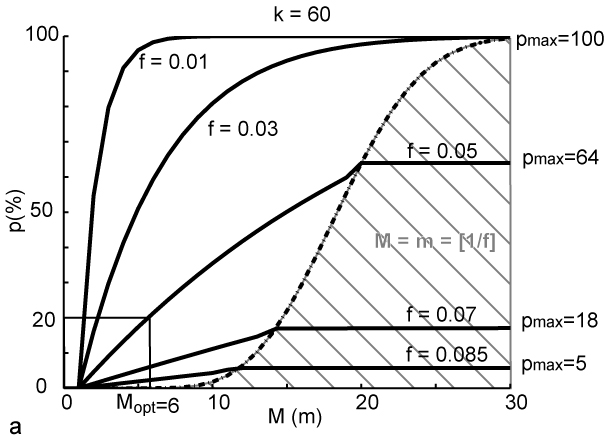
\includegraphics[width=2in]{fig1a.jpg}
  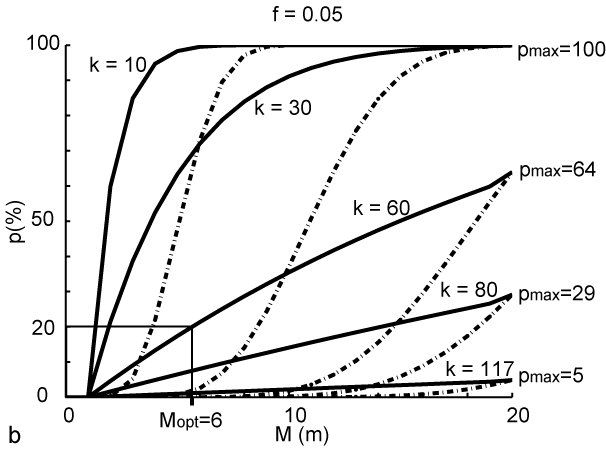
\includegraphics[width=2in]{fig1b.jpg}
  \caption{Evolution of  p$_{max}$ with increasing number of population/sample 
fractions for a) a fixed number  of measurements (k=60) and b) a fixed
relevant  fraction size  (f=0.05).  Solid  lines represent  worst- and
dashed lines best-case scenarios.  The  shaded region on (a) marks the
area where M$\geq$1/f and p is kept constant at p$_{max}$.}
  \label{fig:1}
\end{figure}

Consider a population that consists of M age fractions and define {\it
relevant} fractions to be those fractions that are greater than f. For
a given M  (assuming M$\leq$1/f), the worst-case scenario  is that M-1
of the population fractions are of size f, and one fraction is of size
1-f(M-1).  The probability p that at least one fraction $\geq$f of the
population was missed is given by:

\begin{equation}
  \label{eq:2}
p  =  \sum_{n=1}^{M-A}(-1)^{n-1} \left(  \binom{M-A}{n}  (1-nf)^k +  B
    \binom{M-1}{n-1} ((M-n)f)^k \right)
\end{equation}
with
\begin{eqnarray*}
A & =    & 0~~~~ \mbox{if:} ~ Mf = 1\\
A & =    & 1~~~~ \mbox{if:} ~ Mf \neq 1\\
B & =    & 0~~~~ \mbox{if:} ~ Mf \geq 1\\
B & =    & 1~~~~ \mbox{if:} ~ Mf < 1
\end{eqnarray*}

This is a combinatoric expression where $\binom{x}{y}$ is the binomial
coefficient.   Each term  in the  summation adds  a correction  to the
previous terms. Equation  \ref{eq:2} is derived in Appendix  A.  For a
given  number  of  relevant  fractions  m  (m$\leq$1/f),  a  best-case
scenario can also be calculated (Appendix A):

\begin{equation}
  \label{eq:3}
p  =  \sum_{n=1}^{m}(-1)^{n-1} \binom{m}{n}\left(1-\frac{n}{m}\right)^k
\end{equation}

Exploration of equations  \ref{eq:2} and \ref{eq:3} over M  and m, and
for different values of f and  k, is shown in Figure \ref{fig:1}.  The
maximum number of (relevant)  fractions for which Equations \ref{eq:2}
and \ref{eq:3} are valid  is 1/f.  At larger values of M  (or m), p is
kept  constant.  The shaded  region on  Figure \ref{fig:1}a  marks the
area where this  is the case.  One way to  reduce the probability that
fractions  $\geq$f  are missed  when only  k grains  are dated  is to
reduce the  number of bins in  the sample histogram.   For example, if
k=60, f=0.05,  and p=20\%,  then M$_{opt}$=6 (Figure  \ref{fig:1}).  A
detrital age-histogram that is constructed in this way conveys as much
information about  the population as  can be inferred from  the sample
and is statistically  "allowed" by p and f.  However,  it is less well
suited  for  showing  the  sample  distribution.   Therefore,  such  a
histogram should  be used in  conjunction with markers for  the sample
data,    or    better    still,    a    probability    density    plot
\cite{silverman1986}.  Such a combined  plot carries an optimal amount
of  information:  the histogram  represents  the  population with  the
resolution that  the data and the  parameters p and f  allow, while at
the same time, the probability density plot represents the data itself
and   the  uncertainties   that   are  associated   with  it   (Figure
\ref{fig:2}). M$_{opt}$ usually is a rather small number, much smaller
than commonly used guidelines for the number of histogram bins such as
Sturges' rule \cite{sturges1926,scott1992}.  Using M$_{opt}$ will tend
to oversmooth the histogram, so  although it theoretically is a viable
way  to reduce  the chance  of  missing significant  fractions of  the
population, there  are better methods  for dealing with  datasets that
contain fewer than the  optimal number of measurements.  These methods
are  discussed   in  the  following  paragraph   and  the  Conclusions
section.

\begin{figure}[here]
  \centering
  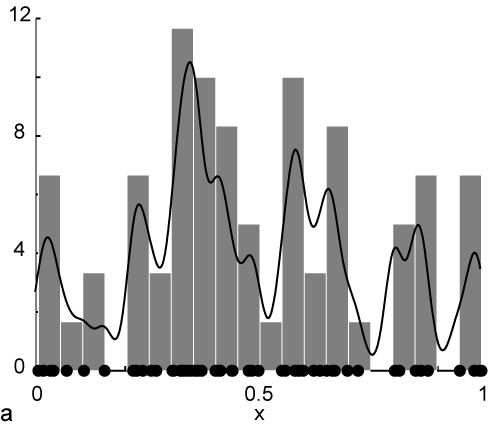
\includegraphics[width=2in]{fig2a.jpg}
  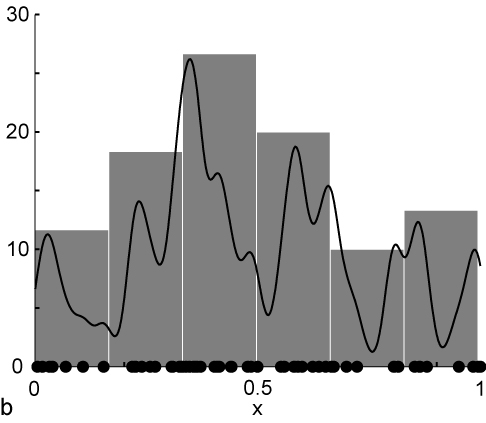
\includegraphics[width=2in]{fig2b.jpg}
  \caption{As shown in Figure \ref{fig:1}, at most M$_{opt}$=6 bins are allowed
  in a  sample histogram in order  to reduce the chance  that at least
  one fraction f$\geq$0.05 is missed of a perfectly uniform population
  (worst-case scenario) to less than p=20\%.  The black dots represent
  the  60  samples.  In  histogram  a,  M=20$\geq$M$_{opt}$.  In  this
  particular  example, three  bins  are empty,  amounting  to a  total
  fraction 0.15 of the population.   When the data are grouped into 20
  bins, this occurs  64\% of the time.  In  histogram b, M=M$_{opt}$=6
  and, for exactly the same sample, no fraction $\geq$ 0.05 is missed.
  Only 20\% of the histograms with  6 bins will have an empty fraction
  in their worst-case scenario, which corresponds to five fractions of
  size 0.05 and one of  size 0.75. While using M$_{opt}$ theoretically
  is a  valid way  to prevent relevant  fractions of being  missed, it
  will  generally  yield oversmoothed  histograms  and  be of  limited
  practical  use.  Instead, it  is better  to simply  report f$_{act}$
  and/or p$_{max}$ along with the data.}
  \label{fig:2}
\end{figure}

Rather than reducing m, a much better way to reduce p is to increase k
or f.  We now define p$_{max}$ as the maximum value of p, reached when
M=m=[1/f],  where  square  brackets  mark truncation  to  the  nearest
integer.    The  equation  for   p$_{max}$  is   a  special   case  of
(\ref{eq:2}):

\begin{equation}
  \label{eq:4}
p_{max}  =  \sum_{n=1}^{[1/f]}(-1)^{n-1} 
            \binom{[1/f]}{n}  (1-nf)^k
\end{equation}

Figure \ref{fig:3} shows the evolution of p$_{max}$ as a function of f
and k. Note the discrete "knee" in the p$_{max}$ vs.  f curve wherever
M = 1/f.  Figure \ref{fig:3} can be used for a quick assessment of the
number of  grains that are needed  for a provenance study,  and of the
risk  of information  loss that  is  caused by  smaller samples.   For
example, if  60 grains are dated, then  $p_{max}$=64\%.  Therefore, in
the  worst-case  scenario (which,  at  m=20,  is  a perfectly  uniform
population) there is 64\% chance that at least one fraction $\geq$0.05
of the population is missed.   This is a dramatically different result
from   the   5\%  probability   suggested   by  Equation   \ref{eq:1}.
Furthermore, the actual fraction f$_{act}$  that we can be sure not to
have missed with 95\% certainty is not 0.05, but 0.085, as can be read
from  Figure  \ref{fig:3}.   Finally,  and perhaps  most  importantly,
Figure \ref{fig:3} also shows that  in order to be 95\% confident that
no  fraction $\geq$0.05  was missed,  at  least k=117  grains must  be
dated. Table 1 can be used  to choose k, the number of grains required
to lower  p and f to some  desired limits. If fewer  than this optimal
number of grains have been dated,  Table 2 can be used to estimate the
actual levels  of p and  f that have  been achieved with that  k.  The
same table  also lists  the value of  $M_{opt}$ in the  unlikely event
that the user  prefers to reduce the resolution  of the age histogram,
rather than  to increase the  desired p and/or  f.  Table 1  should be
used  before embarking  on a  provenance study  to determine  how many
grains  are  needed.  Alternatively,  Table  2  can  be used  for  the
interpretation of provenance data with less than the optimal number of
grains.  For example, if only 30  grains have been dated, Table 2 says
that  f$_{act}$=0.15 is  the smallest  fraction not  missed at  a 95\%
confidence level.  Likewise, there is  20\% chance of missing at least
one fraction representing $\geq$0.12  of the total population, and the
probability of missing at least  one fraction $\geq$0.1 when 30 grains
were dated is 37\%.  Finally, to reduce the chance of missing at least
one fraction $\geq$0.2 of the  population to less than 10\%, and still
only  use   30  grains,  the  age-histogram  cannot   have  more  than
M$_{opt}$=5  bins.  As an  alternative to  Figure \ref{fig:3},  and to
Tables 1 and 2, an online web-form \cite{webform} is available for the
calculation of k, p$_{max}$, f$_{act}$ and M$_{opt}$.

\setcounter{table}{1}
\begin{minipage}[c]{\textwidth}
 Table 1:\\  The adequate number  of grains (k)  as a function  of the
 desired probability  (p) of missing at  least one fraction  $\geq$f of a
 worst-case population.\\
 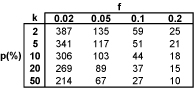
\includegraphics[width = 3in]{table1.jpg}
\label{tab:1}
\end{minipage}

 \section{More realistic populations}\label{sec:realistic}

As  was  shown  in the  first  part  of  the  paper, of  all  possible
populations,  the most  difficult  to sample  is  a perfectly  uniform
distribution,  where each age  fraction is  of the  same size.   It is
sufficient to date k grains,  according to Figure \ref{fig:3}, Table 1
or  the web-form  \cite{webform}, to  reduce f  and p  to  the desired
levels.  However, most  naturally-occuring populations differ from the
worst-case  distribution  and it  is  less  likely that  statistically
significant fractions of such populations might be missed in a sample.
As a consequence, fewer grains  need dating to achieve the same levels
of f and p.  A  number of numerically-generated random populations are
discussed next, followed by some real detrital age-spectra.\\

\subsection{Synthetic populations}\label{sec:numerical}

In this section, we will try to find the minimum number of grains that
have to be  dated to adequately represent an  "average" population, as
opposed  to  the best-  and  worst-case  populations  of the  previous
section.  We will assume that all possible detrital populations of the
geologic record are equally likely  to occur.  Such populations can be
synthetically generated by  randomly selecting multinomial proportions
from a uniform distribution. This procedure is illustrated in Appendix
B.  Thus, for any specific number  of fractions M, we generate a large
number of  random populations (e.g.   1000).  For each  population, we
construct  a large  number (e.g  200)  of random  samples (again,  see
Appendix  B for details).   For each  sample, the  relevant population
fractions are tested to see if the sample contains at least one "grain
age" that falls within it.  If  at least one of the relevant fractions
is empty,  the test has  failed.  The ratio  of the number  of samples
that  failed the test  to the  total number  of samples  represents an
estimate of p. This process is repeated for a range of values for M.

\begin{figure}[here]
  \centering
  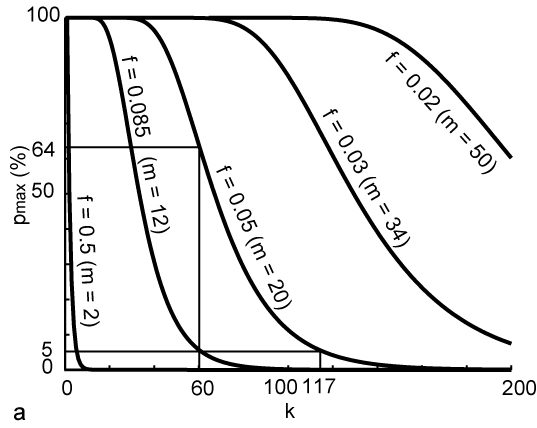
\includegraphics[width=3in]{fig3a.jpg}
  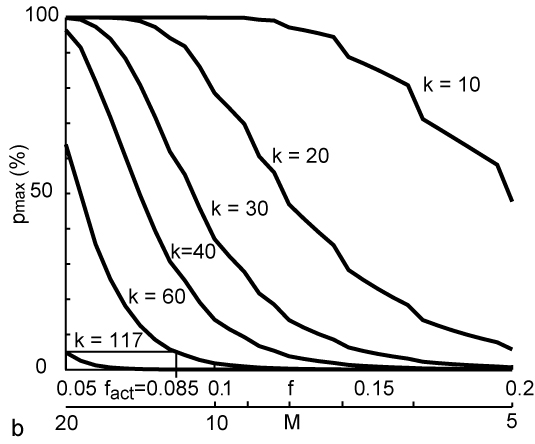
\includegraphics[width=3in]{fig3b.jpg}
  \caption{Graphs that allow a quick assessment of the number of grains
  (k)  needed to  push the  chance of  missing at  least  one fraction
  $\geq$f of a worst-case population below $p_{max}$, a) as a function
  of  the  number  of grains  (k)  and  b)  the number  of  (relevant)
  fractions (M) or their size (f).}
  \label{fig:3}
\end{figure}

Figure \ref{fig:4}  shows the  result of this  procedure for  k=60 and
f=0.05.  For M ranging from one  to 100, 1000 populations of that size
were created.  For each of  these populations, 200 samples of k random
numbers were  generated.  For  each value of  M, a  5, 50, 95,  99 and
100\% percentile  was computed  from the p-values  of its  1000 random
populations.   The higher  its  "percentile", the  closer a  synthetic
population  is  to  a   uniform  distribution.   For  example,  a  "99
percentile" population is likely to be strongly multimodal, while a "5
percentile" population  would be more  unimodal.  All future  plots in
this paper  that are derived  from plots like Figure  \ref{fig:4} will
only  consider the  95\%  percentile populations.   That said,  Figure
\ref{fig:4}  is the numerical  "intermediate-case" analogue  to Figure
\ref{fig:1}.  p  reaches a maximum  value at M$\approx$35, and  not at
M=20, which  would be  the expected result  when only  considering the
fact that at M=20 (=1/f), the number of relevant fractions (m) reaches
a maximum.  The reason why the peak is located at a higher M is that p
is not only a function of m,  but the result of a tradeoff between the
number  of  relevant  fractions  (m)  and the  total  portion  of  the
population  that  is covered  by  these  fractions,  where the  latter
parameter   steadily  decreases  with   increasing  M.    From  Figure
\ref{fig:4} (which,  as discussed before,  is only valid for  k=60 and
f=0.05), the  chance of missing  at least one fraction  f$\geq$0.05 in
the median population  is 10\%; p$\leq$18.5\% in 95\%  of the randomly
generated  populations; p$\leq$25\%  in 99\%  of the  populations; and
p$\leq$  30\%  in  all  1000  populations.   Not  surprisingly,  these
probabilities  are   significantly  less  than  the   64\%  which  was
calculated for the worst-case scenario for the same values of k, f and
p with Equation \ref{eq:4}.  However, even for samples from the median
synthetic  population, the  chance of  missing at  least  one fraction
$\geq$0.05 is more than the 5\%  which was the result of the erroneous
use of Equation  \ref{eq:1}.  Only in little over  5\% of all randomly
generated  populations there  is less  than 5\%  chance of  missing at
least one  fraction $\geq$0.05 of  the population when 60  grains were
measured.   In addition  to  a numerical  analogue  to the  analytical
parameter $p_{max}$, it is also possible to obtain a numerical version
of  $M_{opt}$  (Figure \ref{fig:4}).   This  value  will generally  be
larger  than its  analytical equivalent  for the  worst-case scenario.
For example,  to reduce  the chance of  missing at least  one fraction
$\geq$0.05  of the  population  to  less than  5\%,  while still  only
measuring 60 grains, the maximum  number of fractions that can be used
in the age-histogram is M$_{opt}$=6  (as opposed to M$_{opt}$=2 in the
worst-case scenario).

\begin{figure}[here]
  \centering
  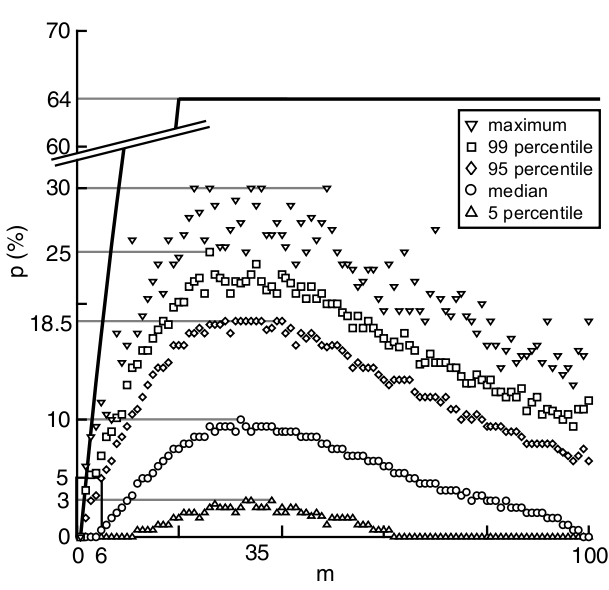
\includegraphics[width = 8in]{fig4.jpg}
   \caption{The random uniform numerical analogue to Figure \ref{fig:1},
for  k=60 and  f=0.05.   The  solid black  line  gives the  worst-case
probability from  Figure \ref{fig:1}. The  different symbols represent
different  levels of  uniformity.   The higher  its "percentile",  the
closer  a synthetic  population  is to  a  uniform distribution.   For
example,  a "99  percentile" population  is likely  to  be multimodal,
while a "5 percentile" population would be nearly unimodal.}
  \label{fig:4}
\end{figure}

By  tracing the evolution  of the  numerical $p_{max}$  with k  and f,
Figure  \ref{fig:5}  illustrates  the  numerical  analogue  to  Figure
\ref{fig:3}.  It  allows a  quick estimation of  the number  of grains
that are  required for certain  key values of  f and p.   For example,
when 95\% confidence is desired that no fraction $\geq$0.05 is missed,
and  this for  95\% of  all randomly  generated populations,  at least
$\sim$95 grains have to be dated.   This estimate is less than the 117
grains  which are necessary  in the  worst-case scenario,  but greater
than the  60 grains that Equation  \ref{eq:1} implies.  Alternatively,
when 60  grains are  dated, we  can be 95\%  certain that  no fraction
f$_{act} \geq$0.07  was missed.  As  might be expected,  the numerical
estimate falls in between the worst-case scenario (f$_{act}$=0.85) and
the result from Equation \ref{eq:1} (f=0.05).

 \begin{figure}[here]
   \centering
   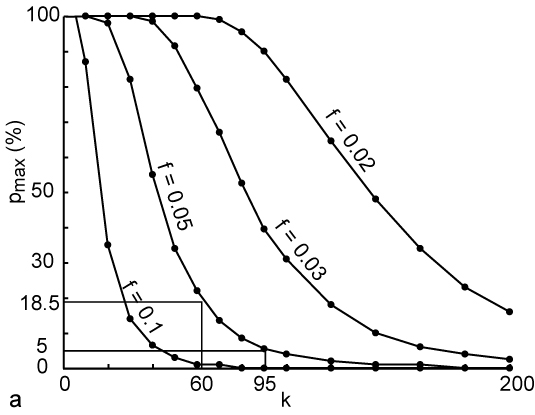
\includegraphics[width = 3in]{fig5a.jpg}
   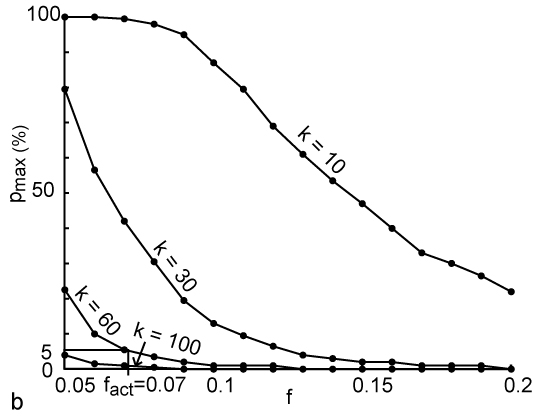
\includegraphics[width = 3in]{fig5b.jpg}
   \caption{The numerical 
   analogue to Figure \ref{fig:3}, this  plot allows a quick lookup of
   the  maximum  probability  (p$_{max}$)  of  missing  at  least  one
   fraction $\geq$f  of a "95 percentile" synthetic  population when k
   grains are dated.}
   \label{fig:5}
 \end{figure}

\subsection{Case studies of real populations}\label{sec:natural}

Now that the theoretical foundations  have been built to calculate the
number  of grains  required  for a  statistically adequate  provenance
study, they will be tested on real data.  Unfortunately, no population
is  ever completely  known (certainly  not  if we  consider that  most
published  provenance  studies  work  with  fewer than  117  ages  per
sample). Therefore, two relatively  large published detrital data sets
will be  used as a  proxy for the  populations that they  were sampled
from.   By randomly  selecting numbers  from these  "populations" with
replacement,  we can  generate synthetic  samples.  This  procedure is
similar  to   what  is  called  "bootstrapping"   in  the  statistical
literature \cite{efron1993}.\\

Avigad  {\it  et  al.}   \cite{avigad2003}  published  a  set  of  157
concordant  single zircon U/Pb  ages from  the Early  Paleozoic Nubian
Sandstone.  The vast  majority of these grains are  of Pan-African age
(900-540  Ma)  with  relatively  few  older  grains.   Therefore,  the
population is relatively "easy"  to sample (Figure \ref{fig:6}).  1000
"bootstrap samples" of  k numbers were selected from  the data set for
each value of M between 1 and 50, where the latter value is assumed to
be the  highest number of bins  that one would  ever want to use  in a
grain-age  histogram.   Similar to  the  algorithm  that  was used  in
section \ref{sec:numerical},  the proportion of the  1000 samples that
miss  at  least  one  of  the  relevant  fractions  (f$\geq$0.05)  was
calculated.  This exercise  was done for k=60, k=95  and k=117 (Figure
\ref{fig:6}).  The p$_{max}$ vs.  M  curve of this figure is much more
irregular than that of Figures \ref{fig:4} and \ref{fig:1}, because it
represents only one, irregular population,  and not the composite of a
thousand  random  distributions (Figure  \ref{fig:4}),  or one  smooth
uniform analytical  distribution (Figure \ref{fig:1}).   For k=60, the
maximum value for p is 8.8\%.  As expected, this is less than the 64\%
predicted  by  Equation  \ref{eq:4},  but  almost  twice  as  much  as
predicted  by Equation \ref{eq:1}.   The fact  that even  samples from
this "easy" population  have $\geq$5\% chance of missing  at least one
fraction  $\geq$0.05 is  another confirmation  that 60  grains  is not
enough to attain the degree  of adequacy many would consider necessary
for a good  provenance study.  The maximum probability  of missing any
fraction $\geq$0.05 is reduced to  1.5\% when 95 grains are dated, and
if k=117, p is only 0.9\%.

 \begin{figure}[here]
   \centering
   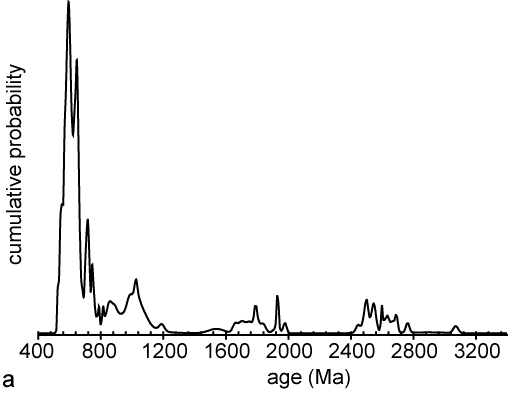
\includegraphics[width = 3in]{fig6a.jpg}
   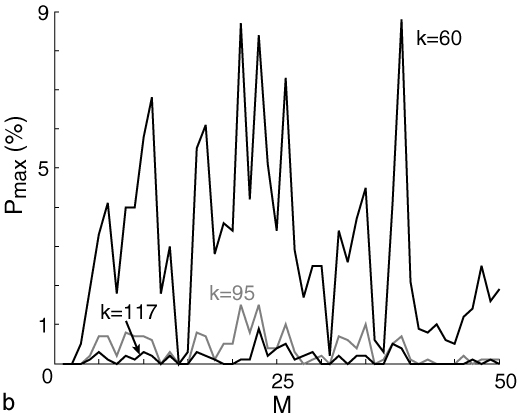
\includegraphics[width = 3in]{fig6b.jpg}
   \caption{a) probability density plot of the Nubian Sandstone
   \cite{avigad2003}  and  b)   the  result  of  numerical  resampling
    experiments for different numbers of grains (k), for f=0.05.}
   \label{fig:6}
 \end{figure}

As  an example  that  is closer  to  the worst-case  scenario, we  now
consider a dataset of  155 $^{40}$Ar/$^{39}$Ar ages on lunar spherules
collected by Apollo 14  \cite{culler2000}.  The age-histogram of these
data  is more  evenly distributed  than was  the case  for  the Nubian
Sandstone (Figure  \ref{fig:7}).  The maximum  probability for missing
at  least one fraction  $\geq$0.05 when  only 60  grains are  dated is
28\%.  When 95  grains are dated, the probability  of missing at least
one  fraction $\geq$0.05  is reduced  to 3.7\%.   Finally,  dating 117
grains results in p=1.2\%.

 \begin{figure}[here]
   \centering
   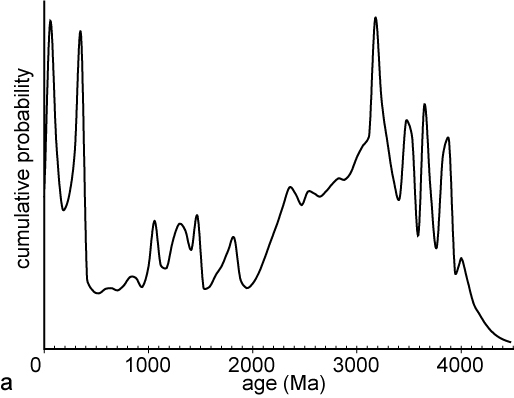
\includegraphics[width = 3in]{fig7a.jpg}
   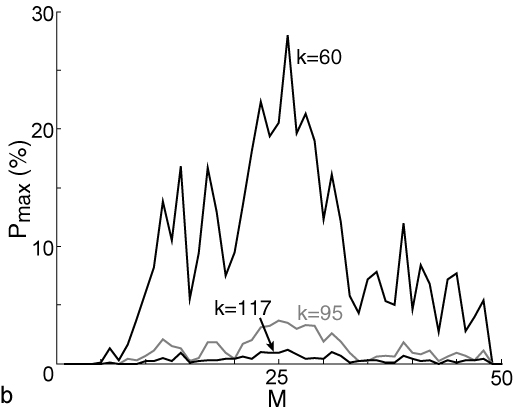
\includegraphics[width = 3in]{fig7b.jpg}
   \caption{Same as Figure \ref{fig:6}, but for the lunar impact spherules data
   \cite{culler2000}.}
   \label{fig:7}
 \end{figure}

\section{Conclusions and recommendations}

\begin{itemize}
\item The optimal number of grains  that should be dated of a detrital
provenance sample can  be looked up from Table  1, Figure \ref{fig:3},
or the web-form  \cite{webform}.  To be 95\% certain  that no fraction
$\geq$0.05 of the  population was missed, 117 grains  should be dated.
This is a  fairly large number, often too  high perhaps for analytical
methods such  as fission-track, (U-Th)/He, or  TIMS.  117 measurements
may  be   more  readily  achievable  with   the  ion-microprobe  (e.g.
\cite{avigad2003})        or        laser       ablation        ICP-MS
(e.g. \cite{dickinson2003}).
\item If there  exists some prior knowledge about  the population that
indicates it is not uniformly distributed, a risk can be taken to date
fewer that the optimal number  of grains, by using Figure \ref{fig:5}.
To  be 95\% certain  that no  fraction f$\geq$0.05  was missed,  it is
recommended  that this  number be  no less  than 95.   However, dating
fewer grains limits the possibility to rigorously calculate and report
p and f.
\item It is  definitely not the purpose of this  paper to suggest that
studies reporting  fewer than  117 single-grain measurements  would be
scientifically wrong.   The purpose of some provenance  studies may be
to prove the {\it presence} of one or more specific age fractions in a
detrital population.   Once these fractions have been  found, there is
no reason  to date  more grains.  It  is only when  provenance studies
discuss  the {\it  absence}  of certain  age  fractions that  counting
statistics come into play.  Even then,  it may not be possible to date
as many as  117 grains for technical, financial  or other reasons.  If
fewer than  117 grains were  dated per sample, or  when age-histograms
must be  interpreted from  published studies that  use fewer  than the
optimal  number of  grains, the  actual  p$_{max}$ and  f values  that
result  from  using the  available  number  of  grain ages  should  be
reported.  For example: if only 60 grains were dated, it is sufficient
to  report  that the  maximum  probability  of  missing at  least  one
fraction greater than  0.05 is p$_{max}$=64\%, {\it or}  that there is
95\% confidence that no  fraction f$_{act}\geq$0.085 was missed.  Note
that  the  latter definitely  sounds  better  than  the former.   Such
information   can  be  obtained   from  Equation   \ref{eq:4},  Figure
\ref{fig:3}, Table  2, or the web-form \cite{webform}.   In theory, an
alternative solution to changing p and f would be to reduce the number
of bins of the age histogram to M$_{opt}$, according to Table 2 or the
web-form \cite{webform}.  However, M$_{opt}$ is typically a low number
which would over-smooth the histogram.
\end{itemize}

\begin{minipage}[c]{\textwidth}
Table 2\\ f$_{act}$, p$_{max}$ and  M$_{opt}$ as a function of k.\\
   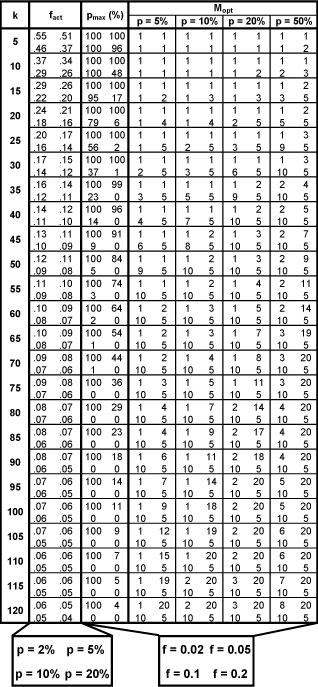
\includegraphics[height = 7.5in]{table2.jpg}\\
\label{tab:2}
Given a specified  number of grains (k), this  Table shows f$_{act}$ -
the  smallest population  fraction that  has not  been missed  with at
least p\%  certainty - for four  values of p; p$_{max}$  - the maximum
probability of missing  at least one fraction $\geq$f  of a worst-case
population - for four values of  f; and M$_{opt}$ - the largest number
of bins  that are less than p\%  likely to miss at  least one fraction
$\geq$f of the worst-case population - for four values of f and p.
\end{minipage}

\section*{Appendix A: derivation of Equations \ref{eq:2} and \ref{eq:3}}

\begin{minipage}[c]{\textwidth}

Of  all   possible  populations,   those  with  a   perfectly  uniform
distribution require the collection of  the largest sample in order to
be certain  that no significant  fractions have been missed.   We will
consider the case where there  are M=20 such fractions.  This case can
easily be generalized to any M.  For a perfectly uniform distribution,
each of the 20 fractions equals exactly f=0.05.

  \begin{center}
  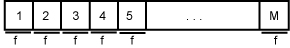
\includegraphics[width=10cm]{A1.jpg}  
  \end{center}

If we  are interested in  only one of  these fractions, e.g.   \#1 (in
subsequent figures, the shaded  box(es) indicate(s) the fraction(s) of
interest), then the probability of missing this fraction is p=1-f. The
probability that  this occurs  for each  one of k  experiments is  p =
(1-f)$^k$. This is  the probability calculated by Dodson  {\it et al.}
\cite{dodson1988}, and given by Equation \ref{eq:1}.

  \begin{center}
  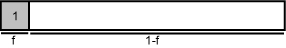
\includegraphics[width=10cm]{A2.jpg}  
  \end{center}

However, if we are not just interested in one particular fraction, but
in all 20  fractions, the probability of missing at  least one of them
is much larger. It is the probability of missing:
\end{minipage}

\begin{minipage}[c]{\textwidth}

  \begin{center}
  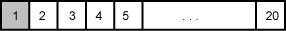
\includegraphics[width=10cm]{A3.jpg}\\
  \mbox{or:}\\
  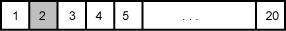
\includegraphics[width=10cm]{A4.jpg}\\
  \mbox{or}\\
  \mbox{...}\\
  \mbox{or}\\
  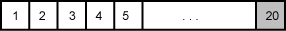
\includegraphics[width=10cm]{A5.jpg}  
  \end{center}

In combinatoric terms:

\begin{equation}
  \label{eq:first_approx}
  p  = \binom{20}{1}(1-f)^k
\end{equation}

While better than (\ref{eq:1}), this is still not the equation that we
want,   because   the  probability   that   any   two  fractions   are
simultaneously missed is counted twice,  causing an estimate of p that
is too high.  Therefore, the following situations:
\end{minipage}

\begin{minipage}[c]{\textwidth}

  \begin{center}
  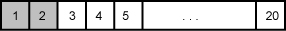
\includegraphics[width=10cm]{A6.jpg}\\
  \mbox{or}\\
  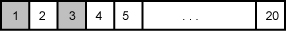
\includegraphics[width=10cm]{A7.jpg}\\
  \mbox{or ...}
  \end{center}

have to be subtracted from Equation \ref{eq:first_approx}. This
gives rise to the following expression:

\begin{equation}
  \label{eq:second_approx}
  p  = \binom{20}{1}(1-f)^k - \binom{20}{2}(1-2f)^k
\end{equation}

Equation  \ref{eq:second_approx}   is  a  better   approximation  than
Equation  \ref{eq:first_approx},   but  the  probability   that  three
fractions are missed  at the same time is  subtracted twice, resulting
in too  low an estimate  for p.
\end{minipage}

\begin{minipage}[c]{\textwidth}
  \begin{center}
  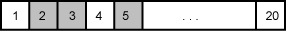
\includegraphics[width=10cm]{A8.jpg}  
  \end{center}

Therefore, a correction is added to (\ref{eq:second_approx}), becoming
a third-order approximation:

\begin{equation}
  \label{eq:third_approx}
  p  = \binom{20}{1}(1-f)^k - \binom{20}{2}(1-2f)^k + \binom{20}{3}(1-3f)^k
\end{equation}

This  equation will again  overestimate p  because the  probability of
simultaneously missing  four fractions is counted twice.   It is clear
by  now  that  this  process  of  iterative  corrections  to  Equation
\ref{eq:first_approx} can be repeated  until we have corrected for the
probability that all twenty fractions are missed:

\end{minipage}

\begin{minipage}[c]{\textwidth}

  \begin{center}
  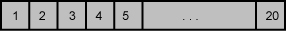
\includegraphics[width=10cm]{A9.jpg}  
  \end{center}

This probability equals $\binom{20}{20}(1-20f)^k = 0$, a trivial result.
Adding it to the 19 previous corrections yields:

\begin{eqnarray}
  p  & = & \binom{20}{1}(1-f)^k - \binom{20}{2}(1-2f)^k + ... 
           - \binom{20}{20}(1-20f)^k\\
  ~  & = & \sum_{n=1}^{20}(-1)^{n-1} \binom{20}{n}  (1-nf)^k
  \label{eq:twentieth_approx}
\end{eqnarray}

or, generalizing by replacing 20 with M:

\begin{equation}
  \label{eq:a0b0}
\sum_{n=1}^{M}(-1)^{n-1} \binom{M}{n}  (1-nf)^k\\
\end{equation}

Equation \ref{eq:a0b0}  is a  special instance of  Equation \ref{eq:2}
for A = 0 and B = 0.  This form gives the correct value for p when the
relevant fractions exactly add up  to 100\% of the population (i.e.  M
= 1/f).  There are two  situations where the relevant fractions do not
exactly add up to one:

\end{minipage}

  \begin{center}
  A = 1, B = 0:\\ 
  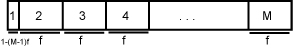
\includegraphics[width=10cm]{A10.jpg}\\  
  or  A = 1, B  = 1:\\ 
  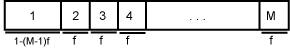
\includegraphics[width=10cm]{A11.jpg}
  \end{center}

The derivation  of p  for these cases  is completely analogous  to the
derivation of Equation \ref{eq:a0b0}.  Equation \ref{eq:2}
is a generalization that takes care of all possibilities.\\

\noindent In addition to the worst-case  scenario, a best-case scenario can also
be considered  given a certain  number of relevant fractions  (m).  If
the number of  relevant fractions is not known,  the lowest possible p
is always associated with a delta function (one single age component).
For the latter population p  equals zero, which is an information-free
trivial  result.  For example,  if m  = 3,  the best-case  scenario is
given by:


\begin{minipage}[c]{\textwidth}

  \begin{center}
  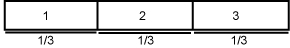
\includegraphics[width=10cm]{A12.jpg}\\  
  \end{center}

The derivation  of p  for this case  is completely analogous  to the
derivation of Equation \ref{eq:a0b0} with M = m = 3 and f = 1/3:

\begin{equation}
\label{eq:best_case}
p  =  \sum_{n=1}^{3}(-1)^{n-1} \binom{3}{n}\left(1-\frac{n}{3}\right)^k
\end{equation}

\end{minipage}

\section*{Appendix B: details of the synthetic population generator.}

\begin{minipage}[c]{\textwidth}

Consider a specific value for M (the number of fractions), for example
M=7.  A  population is generated by  selecting an array  of M-1 random
numbers  between  zero and  one,  drawn  from  a uniform  distribution
(x$_i$, with i=1...6). This array  is sorted and padded with a leading
zero and a trailing one, becoming of size M+1.

  \begin{center}
  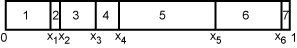
\includegraphics[width=10cm]{B1.jpg}\\  
  \end{center}

The difference between subsequent numbers  in the array is a new array
of size  M (f$_j$, with j=1...7),  in which each  element represents a
fraction of  the total population.  The population,  when generated in
this way, is automatically normalized to one.

  \begin{center}
  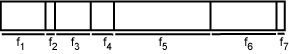
\includegraphics[width=10cm]{B2.jpg}\\  
  \end{center}

Random samples  are generated  by choosing k  (for example  20) random
numbers between zero and one, also from a uniform distribution. On the
following figure, these numbers are marked by black dots.  Each of the
relevant fractions ("boxes") of the population is tested to see if the
sample contains at least one  number ("dot") that falls within it.  On
the next figure, the relevant fraction size f is marked by a gray bar.
If  at least  one of  the relevant  fractions is  empty, the  test has
failed. This is the case for our example, since the third box is empty
and  f$_3\geq$f. Note that  fraction \#7  is also  empty, but  this is
irrelevant because f$_7<$f.

  \begin{center}
  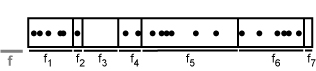
\includegraphics[width=12cm]{B3.jpg}\\  
  \end{center}

\end{minipage}

For each  population, the ratio of  the number of  samples that failed
the test to the total number  of samples represents one estimate of p.
This  procedure  is  repeated  for  a large  number  of  synthetically
generated populations.  The iterative  process becomes of  third order
when a range of M values is evaluated (Figure \ref{fig:4}).

\section*{Acknowledgements}

Many  thanks   to  Jianmei  Wang  for   mathematical  discussions  and
assistance; to  Mike McWilliams,  Raymond Jonckheere and  Paul Switzer
for  useful reviews of  initial drafts  of the  paper; and  to Anthony
Koppers and Keith Sircombe  for insightful and constructive reviews of
the submitted  manuscript, which  greatly improved the  readability of
the paper.

\begin{thebibliography}{}

\bibitem{dodson1988} M.H.  Dodson,  W.  Compston, I.S.  Williams, J.F.
Wilson, A search for ancient detrital zircons in Zimbabwean sediments,
J.  Geol. Soc. London 145 (1988) 6, 977-983.

\bibitem{morton1996}  A.C.   Morton,   J.C.   Claou\'{e}-Long  and  C.
Berge, SHRIMP constraints on sediment provenance and transport history
in the Mesozoic Statfjord Formation,  North Sea, J.  Geol. Soc. London
153 (1996) 6, 915-929.

\bibitem{cawood2001}  P.A. Cawood  and  A.A. Nemchin,  Paleogeographic
development  of  the East  Laurentian  margin;  constraints from  U-Pb
dating   of  detrital  zircons   in  the   Newfoundland  Appalachians,
Geol. Soc. Am. Bull. 113 (2001) 9, 1234-1246.

\bibitem{rahl2003}   J.M.   Rahl,   P.W.   Reiners,   I.H.   Campbell,
S. Nicolescu and C.M.  Allen, Combined single-grain (U-Th)/He and U/Pb
dating of detrital zircons from the Navajo Sandstone, Utah, Geology 31
(2003) 9, 761-764.

\bibitem{grimmer2003}  J.C. Grimmer,  L. Ratschbacher,  M. McWilliams,
L. Franz, I. Gaitzsch, M.  Tichomirowa, B.R. Hacker and Y. Zhang, When
did   the    ultrahigh-pressure   rocks   reach    the   surface?    A
$^{207}$Pb/$^{206}$Pb   zircon,    $^{40}$Ar/$^{39}$Ar   white   mica,
Si-in-white  mica,   single-grain  provenance  study   of  Dabie  Shan
synorogenic foreland sediments, Chem. Geol. 197 (2003) 87-110.

\bibitem{silverman1986}B.W.    Silverman,   Density   estimation   for
statistics and data analysis, Chapman \& Hall, London, 1986, 175 pp.

\bibitem{sturges1926} H.A.   Sturges, The choice of  a class interval,
J. Am. Stat. Assoc. 21 (1926) 65-55.

\bibitem{scott1992}  D.W.  Scott,  Multivariate  density estimation  :
theory, practice,  and visualization, Wiley,  New York, NY,  1992, 317
pp.

\bibitem{webform} \mbox{http://pangea.stanford.edu/research/noble/provenance}

\bibitem{efron1993} B. Efron and R. Tibshirani, An introduction to the
bootstrap (1993) Chapman \& Hall, New York, NY, 436 pp.

\bibitem{avigad2003}  D.   Avigad, K.   Kolodner,  M.  McWilliams,  H.
Persing,  T.   Weissbrod,  Provenance  of northern  Gondwana  Cambrian
sandstone revealed by detrital zircon SHRIMP dating, Geology 31 (2003)
3, 227-230.

\bibitem{culler2000} T.S.  Culler, T.A.  Becker, R.A.  Muller and P.R.
Renne, Lunar  impact history from $^{40}$Ar/$^{39}$Ar  dating of glass
spherules, Science 287 (2000) 5459, 1785-1788.

\bibitem{dickinson2003} W.R. Dickinson and  G.E. Gehrels, U-Pb ages of
detrital zircons  from Permian and  Jurassic eolian sandstones  of the
Colorado   Plateau,  USA:   paleogeographic   implications,  Sediment.
Geol. 163 (2003) 29-66.

\end{thebibliography}

\end{document}
